% CS5228 Group 6: English final-report structure.
% Based on the supplied IEEE conference template.
% Sections I, II, and III are drafted; later sections remain a writing skeleton.
% Replace every prompt and TBD before submission. Keep the course layout.
% Main-text budget (including title, abstract, tables and figures):
% Title/abstract 0.4; Introduction 0.6; Data 0.4; EDA/preprocessing 1.4;
% Methods 1.5; Experimental setup 1.0; Results/discussion 2.0;
% Conclusion 0.3 = 7.6 pages, leaving 0.4 pages of buffer.
% References and the appendix are outside the eight-page main-text limit.
% The outline's rendered length does not predict the completed paper's length.

\documentclass[conference]{IEEEtran}
\usepackage[T1]{fontenc}
\usepackage{cite}
\usepackage{amsmath,amssymb,amsfonts}
\usepackage{graphicx}
\usepackage{textcomp}
\usepackage{xcolor}
\usepackage{booktabs}
\usepackage{tabularx}
\usepackage{url}
\usepackage{placeins}
\usepackage[hidelinks]{hyperref}

% Writing prompts are visible during drafting. Replace them with report prose.
% Set \outlinefalse only after adding complete prose, figures and results.
\newif\ifoutline
\outlinetrue
\newcommand{\guide}[1]{%
  \ifoutline\par\noindent{\small\color{blue!65!black}%
  \textit{Writing prompt: #1}}\par\fi}
\newcommand{\pending}{\textit{TBD}}
\newcommand{\figureplaceholder}[2]{%
  \fbox{\parbox[c][#1][c]{0.91\linewidth}{%
  \centering\small\textit{Figure placeholder}\\[4pt]#2}}}
\newcommand{\field}[1]{\texttt{\detokenize{#1}}}

\title{Predicting Singapore HDB Rental Prices under Temporal Distribution Shift}
% Revise the title if the completed experiments support a different emphasis.
\author{%
  \IEEEauthorblockN{Ox Alpha (Group 6)}
  \IEEEauthorblockA{%
    Li Chengxuan (A0352428A), Mao Huanqing (A0257997Y)\\
    Sun Zekun (A0351314R), Zhang Ziqing (A0223145R)\\
    National University of Singapore}
}

\begin{document}
\maketitle

\begin{abstract}
\guide{Write approximately 150--180 words after the final experiments are
complete. State the practical rental-prediction problem, the dataset and
temporal challenge, the analysis and preprocessing approach, the evaluated
methods, and the selected final model. Give its verified evaluation results
and the most important interpretation. Describe completed work in the past
tense. Do not present progress-report scores as final results.}
\end{abstract}

\begin{IEEEkeywords}
HDB rental prediction, temporal validation, feature engineering, regression,
spatial auxiliary data
\end{IEEEkeywords}

\section{Introduction}
\label{sec:introduction}
% Approximately 0.6 pages in the supplied IEEE conference layout.

\subsection{Motivation and Problem Context}
Accommodation costs place a substantial financial burden on households in
Singapore. As the course overview emphasises, renting can be a practical
necessity for people who are unable or ineligible to purchase housing,
including singles, young couples waiting for a new flat, and foreign
workers~\cite{data_source}. Renters need to judge what their budget can secure
and compare asking rents across properties; landlords and real estate agents
need realistic pricing references. These needs motivate our study of
Housing \& Development Board (HDB) flats. Given a flat's characteristics and
approval month, we predict its monthly rent from historical observations and
assess the reliability of predictions for later periods.

This task presents three challenges. First, rental levels change over time:
in the supplied training data, mean rent rises from SGD~2,121 in 2021 to
SGD~3,036 in 2023, followed by much smaller changes in 2024 and early 2025.
These descriptive averages also reflect the mix of properties observed, so
they do not isolate a causal market effect. Nevertheless, the pattern makes
continued extrapolation of an earlier growth trend questionable. Second,
location and property characteristics are interdependent: town, street,
flat type and floor area may encode overlapping information, while amenity
features may contribute differently across models. Third, repeated feature
vectors and inconsistent derived attributes require careful treatment.
Without identifiers for individual flats or contracts, matching rows cannot
be assumed to represent duplicate transactions.

Useful rental estimates must remain credible when the prediction period
extends beyond the observed market conditions. An underestimated rent can
mislead a tenant's budget, while an overestimated rent can distort property
comparisons or pricing expectations. Moreover, low average error can conceal
poor performance for uncommon flat types or less represented locations.
We therefore consider temporal calibration and subgroup errors alongside
overall accuracy. This framing treats the model as a reference based on
observable attributes, rather than a complete valuation of an individual
flat's condition or contractual terms.

\subsection{Research Questions and Contributions}
We address three questions: (1) how do temporal, spatial and property
patterns inform preprocessing and rent prediction; (2) what additional
predictive value do contextual and historical-rent features provide beyond
the core attributes; and (3) which evaluated model performs most reliably
on later observations, and where do its errors remain largest?

Our work connects exploratory analysis to explicit preprocessing decisions,
compares alternative treatments of repeated records, and evaluates Ridge
regression, CatBoost and a multilayer perceptron under chronological
validation. Feature comparisons retain the same individual validation
records and original rents. Data-dependent transformations and rental-history
summaries are constructed from the training portion of each experiment.
The selected model is assessed through later-period errors and a longer
forecasting-horizon diagnostic, rather than through an aggregate score alone.
These contributions concern the application and evaluation of existing
methods; their value lies in identifying which choices support reliable
prediction for this dataset.

\section{Data and Problem Formulation}
\label{sec:data}
% Approximately 0.4 pages, including Table I.
% Dataset facts below were verified against the repository CSVs and metadata.

\subsection{Prediction Task and Core Data}
The CS5228 competition supplies labelled training records and an unlabelled
test set~\cite{data_source}. We learn a regression function $\hat y=f(x)$,
where $y$ is \field{MONTHLY_RENT} in Singapore dollars (SGD). The ten
supplied predictors describe the approval month, town, block, street, flat
type, flat model, floor area, furnishing status, lease commencement year and
upfront fee. All 150,000 training rows are retained; preprocessing is detailed in
Section~\ref{sec:eda}.

\begin{table}[!ht]
  \caption{Overview of the supplied rental data.}
  \label{tab:data}
  \centering
  \small
  \begin{tabularx}{\columnwidth}{l>{\raggedright\arraybackslash}X>{\raggedright\arraybackslash}X}
    \toprule
    Property & Training data & Test data \\
    \midrule
    Raw records & 150,000 & 50,000 \\
    Rental months & Jan. 2021--Mar. 2025 & Mar. 2025--Jul. 2026 \\
    Supplied predictors & 10 & 10 \\
    Target labels & Available & Unavailable \\
    Final modelling records & 150,000 & 50,000 \\
    \bottomrule
  \end{tabularx}
\end{table}

As Table~\ref{tab:data} shows, the split is predominantly temporal: only
380 test records share March 2025 with the training period; all others are
later. The maximum test horizon is 16 months beyond the last training month.
We assess prediction error primarily with root mean squared error (RMSE) in
SGD; the evaluation protocol is specified in Section~\ref{sec:experiments}.

\subsection{Auxiliary Data Sources}
Six supplied auxiliary datasets cover HDB block metadata, Mass Rapid Transit
(MRT) stations, schools, shopping malls, Certificate of Entitlement
(COE)~\cite{coe_background} prices, and stock prices for major Singapore
companies~\cite{company_directory}. Addresses and coordinates support building attributes and amenity features. The selected
feature set combines core, HDB/MRT and training-only rental-history features.
School and mall features were evaluated but excluded. COE and stock features
were excluded because future observations are unavailable at the prediction
cutoff. Historical snapshot limitations are discussed in Section~\ref{sec:eda}.

% Keep the data summary before figures from the following section.
\FloatBarrier

\section{Exploratory Data Analysis and Preprocessing}
\label{sec:eda}
% Completed from notebooks 01--04 and 06, and the improvement experiment log.

\subsection{Target Distribution and Data Quality}
The 150,000 raw training records contain no missing cells. Monthly rent has
a mean of SGD~2,719, a median of SGD~2,700, and a range of SGD~300 to SGD~7,600.
Its skewness is 0.39. The interquartile-range rule flags 752 records
(0.50\%) as extreme, but the supplied attributes cannot establish that these
are recording errors. We retained them and used all original rents for
evaluation. Ridge and CatBoost learned from raw SGD targets; the MLP
standardised targets within each training fold and converted predictions
back to SGD. No logarithmic target transformation was applied.

Two predictors have no variation: \field{FURNISHED} is always \field{yes},
and \field{FEE} is always zero. We removed both. Raw completeness does not
eliminate the need for missing-value handling: masking invalid ages and
cleaning sentinels in the auxiliary tables introduce missing values later
in the pipeline.

\subsection{Temporal Patterns and Distribution Shift}
Fig.~\ref{fig:time} shows rapid rent growth followed by a flatter period.
Mean rent rises from SGD~2,121 in 2021 to SGD~3,036 in 2023, then changes
less in 2024 (SGD~3,110) and January to March 2025 (SGD~3,142).
The last value covers only three months. The average of the first six
monthly means is SGD~2,079, compared with SGD~3,137 for the final six.
These changes motivate a continuous month index and calendar features, but
also make extrapolating an earlier growth rate a potential source of error.
We therefore trained on earlier months and evaluated on later months, as
specified in Section~\ref{sec:experiments}.
\begin{figure}[t]
  \centering
  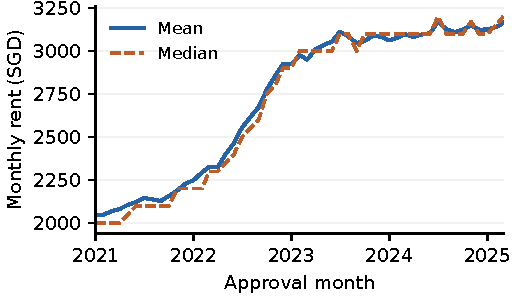
\includegraphics[width=\columnwidth]{figures/eda_temporal.pdf}
  \caption{Monthly mean and median rent across all 150,000 raw training
  records. Faint bars show record counts on the right axis. Early 2025
  covers January to March only.}
  \label{fig:time}
\end{figure}

\subsection{Spatial and Property Patterns}
Rent varies across both property types and towns. After normalising flat-type
labels, median rent increases from SGD~2,100 for two-room flats to SGD~3,000
for five-room and executive flats (Fig.~\ref{fig:flat_type_eda}). Floor area
has a positive raw correlation with rent (Pearson $r=0.33$), although it is
closely related to flat type. We retained both descriptors. Town comparisons
also differ with size: Central has a median rent per square metre of
SGD~41.10, compared with SGD~23.44 in Pasir Ris, whose mean floor area is
larger. These comparisons pool different months and property mixes; they
support location features without identifying causal location premiums.
Rent per square metre was used only for EDA because it contains the target.

\begin{figure}[t]
  \centering
  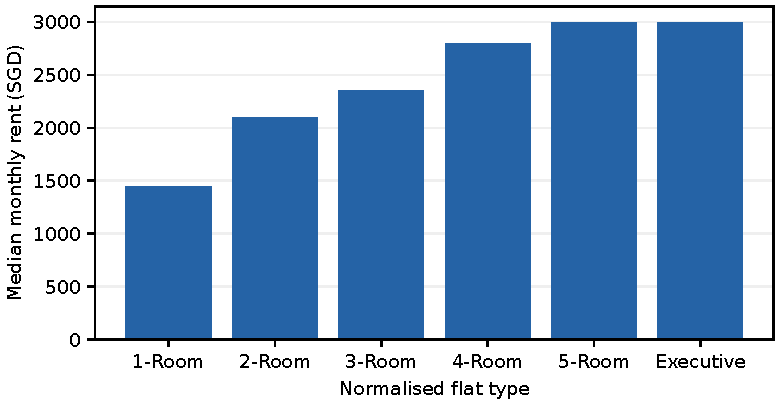
\includegraphics[width=\columnwidth]{figures/eda_flat_type.pdf}
  \caption{Median rent by normalised flat type across the raw training
  records. The comparison does not adjust for month,
  location, or floor area.}
  \label{fig:flat_type_eda}
\end{figure}

\subsection{Core Cleaning and Feature Construction}
We applied Unicode NFKC normalisation, lowercasing, and whitespace cleanup
to categorical fields, removed spaces within block identifiers, and merged
equivalent labels such as \field{4 room} and \field{4-room}. Flat-type
cardinality fell from eleven to six, and street cardinality from 1,146 to
576. Space-separated room labels occur mainly in 2021, so leaving the
spellings separate would mix property categories with formatting changes
over time.

Approval month was parsed into year, month, quarter, a month index, and
sine/cosine seasonal terms. We added town/street and town/block/street
keys for address resolution, an ordered flat-type code, lease age, its
invalidity flag, and $\log(1+\text{floor area})$ alongside raw area.
These transformations give 19 core predictors. Original row IDs and parsed
dates remain alignment and validation fields, not model inputs.

Table~\ref{tab:preprocessing} summarises the cleaning decisions. We checked
the uncertain choices through the preprocessing audit below rather than
assuming that fewer records or more elaborate imputation would improve
prediction.

\begin{table}[t]
  \caption{EDA findings and the corresponding preprocessing decisions.}
  \label{tab:preprocessing}
  \centering
  \small
  \begin{tabularx}{\columnwidth}{p{0.31\columnwidth}X}
    \toprule
    Finding & Decision and justification \\
    \midrule
    Constant fields & Remove fields without predictive variation. \\
    Inconsistent category labels & Normalise case, whitespace and equivalent
    room labels. \\
    Changing rent trend & Encode approval time and validate on later months. \\
    Invalid ages and sentinels & Mask source values, attempt training-only
    address recovery, and retain quality flags. \\
    Identical observations & Retain all rows; exact removal gave negligible
    benefit in controlled validation. \\
    Extreme targets & Retain rents flagged by IQR without evidence of error. \\
    \bottomrule
  \end{tabularx}
\end{table}

\subsection{Preprocessing Audit and Policy Selection}
\label{sec:preprocessing_audit}
The audit in Notebook~06 compared three record policies and two missing-value
treatments using Ridge with $\alpha=10$ and the same 35 core/HDB/MRT features.
Selection used July to December 2023 and January to June 2024, training on
earlier months in each case. Record policies changed the training data only.
The two validation blocks retained all 17,900 and 18,179 original observations,
respectively, and their individual rent labels. Table~\ref{tab:audit_policies}
reports the unweighted mean RMSE across these two windows.

\subsubsection{Repeated observations}
The raw data contain 425 exact matches beyond the first occurrence;
normalisation raises this count to 641. Unit numbers are unavailable, so
identical attributes and rent cannot establish that a transaction was recorded
twice. Multiple units in the same block can share the supplied description.
The audit also found 21,974 repeated feature rows when rent was excluded from
the grouping key. The largest group contains ten observations, and 17,900
feature groups have more than one rent value. These counts distinguish
identical complete records from repeated descriptions with different targets.

We tested retaining all rows, removing exact matches including rent, and
collapsing each identical feature vector to one row with mean rent. The last
policy reduces a group's contribution to training because no group-size
weight is retained. Its mean RMSE was about 603.96 SGD, compared with about
600.80 SGD for the other policies. We did not average validation labels under
any policy.

\begin{table}[t]
  \caption{Notebook~06 preprocessing audit. Mean RMSE in SGD over the two
  earlier selection windows; validation observations are identical for all rows.}
  \label{tab:audit_policies}
  \centering
  \small
  \begin{tabularx}{\columnwidth}{Xrr}
    \toprule
    Training record policy & Median only & Mask/recover \\
    \midrule
    Retain all & 600.803 & 600.808 \\
    Remove exact matches & 600.798 & 600.792 \\
    Collapse to mean rent & 603.965 & 603.962 \\
    \bottomrule
  \end{tabularx}
\end{table}

\subsubsection{Invalid values and address recovery}
Lease age is approval year minus lease commencement year. Ages below zero or
above 100 years are invalid under our rule. One training record is affected:
a November 2021 approval at Bedok block 153B, Bedok South Road, has lease
commencement year 2022. The masking/recovery variant removes this source value
as well as its derived age. HDB maximum floors and completion years at or
below zero are also masked, and completion years are checked for an implied
age outside the same range. Each HDB source field is invalid or missing for
159 training records across eleven addresses. None of these audited numeric
fields is invalid or missing in the supplied test rows. These checks identify
values the model should not use directly; they do not determine corrected
values.

Recovery uses the full normalised town/block/street key. A source attribute
can be recovered only when all valid training values at that address agree.
Conflicting values and unseen addresses retain missing values. We fit the
lookup within each training fold, recheck recovered years against the
approval year, recompute ages, and keep the original invalidity flags.
Remaining numeric gaps use training-fold medians for Ridge and MLP, or
CatBoost's native missing-value handling.

The recovery audit filled no source values in either selection window.
In the first validation block, nine records lacked maximum-floor values and
nine lacked completion years; all remained missing. The second block had no
missing audited source attributes. Since HDB attributes come from a shared
block lookup, another transaction at the same address need not supply an
independent valid value. The result gives no evidence of a predictive gain
from recovering attributes in these windows.

The selection rule preferred retaining records when its mean RMSE was within
1 SGD of the best policy, and preferred masking/recovery when within 0.1 SGD
of the best missing-value treatment. Retention with masking/recovery scored
600.808 SGD, only 0.016 SGD above exact removal with the same treatment.
Its score was also 0.005 SGD above retention with median-only handling.
We selected it to preserve potentially valid transactions and mask invalid
source years, rather than claiming an accuracy improvement from imputation.
These tolerances are practical selection rules, not significance thresholds.
The final pipeline therefore retains all 150,000 training records and every
one of the 50,000 test IDs.

\subsection{Auxiliary Construction and Record Integrity}
The 9,464 HDB block records have unique normalised town, block, and street
keys, with 100\% address coverage in train and test. A many-to-one join adds
coordinates, maximum floor, completion year, postal sector, subzone, planning
area, region, and derived age/quality fields. The eleven blocks with invalid
floor/year sentinels account for the 159 affected training records;
285 block postal codes marked \field{NIL} become missing categories.

Rail data provide current status but no opening dates. We used a fixed proxy
of older line prefixes, excluded eight specified later/future codes, and
deduplicated station names and coordinates, leaving 122 locations. The proxy
excludes TEL and LRT and does not track openings during the rental period.
Haversine distances yield the nearest-station distance and counts within
500 metres and one kilometre. School and mall distances/counts were built
similarly and tested as separate feature groups. They were excluded from the
selected configuration; their snapshots also lack opening histories.

We inspected the supplied Certificate of Entitlement (COE) and stock-price
tables, linked in the project description to COE background
\cite{coe_background} and a Singapore company ranking
\cite{company_directory}. Their cleaned observations were aggregated by
calendar month and shifted by one month. Neither source entered the final
forecasting model: a lag does not establish availability of market observations
throughout the future prediction horizon. We collected no additional data.

The final feature set combines the 35 core/HDB/MRT inputs with four rental-history
fields: past mean rent and count for town/flat-type pairs and for properties.
For training rows, histories exclude the current month and all later months.
Validation and test histories use only rents known in their training data.
The final contract therefore has 39 predictors. Joins check key uniqueness,
row counts, and matching IDs/dates so that adding features cannot silently
change the evaluation population.

\section{Data Mining Methods and Model Development}
\label{sec:methods}
% Approximately 1.5 pages. Reserve substantial space for completed improvements.

\subsection{Reference Predictor and Ridge Baseline}
\guide{Describe the historical town--flat-type median reference and its
fallback rules. Explain why Ridge was selected as a fast baseline for sparse,
correlated predictors. State its feature set and target representation.
Describe how it was applied rather than reproducing textbook derivations.}

\subsection{Candidate Models}
\guide{Describe the alternative models actually evaluated after the progress
report. Possible candidates include boosting models, but do not list a method
as an experiment unless it was run. For each model, explain its suitability,
categorical handling, target representation and principal configuration.
Add verified references for advanced methods. Remove unused candidates.}

\subsection{Completed Model Improvements}
\label{sec:improvements}
\guide{Use this subsection for the improvements completed before submission.
For each change, connect an observed weakness to a specific modification and
its controlled evaluation. Report unsuccessful changes when they explain
why a component was excluded. Do not write this subsection as a plan.}

\subsubsection{Temporal Representation and Calibration}
\guide{Describe any completed changes to linear time trends, piecewise or
capped trends, training windows, recency weights or calibration. Explain how
cutoffs and other choices were selected using historical validation. State
which approach the final model retained. Delete this heading if no such
experiment was completed.}

\subsubsection{Feature Interactions and Auxiliary Information}
\guide{Describe completed tests of time--location or property interactions,
alternative categorical representations, and additional auxiliary feature
groups. Identify retained and rejected features. Distinguish a plausible
explanation from an effect demonstrated by ablation.}

\subsubsection{Tuning and Model Combination}
\guide{Describe completed tuning, early stopping or ensemble experiments.
If an ensemble was used, specify its component models, training protocol and
how its weights were selected without using evaluation labels. Remove this
heading when the final method is a single model with no relevant experiment.}

\subsection{Final Model Specification}
\label{sec:finalmodel}
\guide{Give the selected final model or ensemble, exact feature groups,
target transformation, hyperparameters and training procedure. Explain the
selection criterion. This subsection must describe the implemented final
system, not merely the highest-scoring intermediate run. State the final
refitting procedure and any post-processing used for test predictions.}

\section{Experimental Setup}
\label{sec:experiments}
% Approximately 1.0 pages.

\subsection{Chronological Validation}
\guide{Explain why evaluation must train on earlier rentals and predict later
rentals. Table~\ref{tab:folds} shows the existing expanding windows. Replace
or supplement them if the final protocol changes. State the prediction
horizon and any gap. Explain how final performance was evaluated separately
from tuning, or explicitly disclose reuse of the tuning folds.}

\begin{table}[t]
  \caption{Existing chronological validation windows. Update to match the
  final evaluation protocol.}
  \label{tab:folds}
  \centering
  \small
  \begin{tabularx}{\columnwidth}{lXX}
    \toprule
    Fold & Training through & Validation period \\
    \midrule
    1 & Jun. 2023 & Jul.--Dec. 2023 \\
    2 & Dec. 2023 & Jan.--Jun. 2024 \\
    3 & Jun. 2024 & Jul. 2024--Mar. 2025 \\
    \bottomrule
  \end{tabularx}
\end{table}
\guide{The current validation blocks span 6, 6 and 9 months, while the
maximum test prediction distance is 16 months after the last training month.
Describe any completed longer-horizon evaluation, or acknowledge the horizon
limitation. A fold already used to choose models is not an untouched holdout.}

\subsection{Training-Fold Preprocessing and Leakage Controls}
\guide{Describe how numerical imputation, scaling, categorical vocabularies
and infrequent-category grouping were fitted inside each historical training
fold. Explain any model-specific exceptions. Exclude target-derived inputs.
State how unknown categories and auxiliary missingness were handled.}

\subsection{Hyperparameter Selection and Reproducibility}
\guide{Report the actual search strategy, search space, validation criterion,
random seeds, software versions and relevant resource constraints. The
existing Ridge search uses alpha in \{0.1, 1, 10, 100\}; update this if expanded.
Summarise decisive settings in the main text and put the full grid in the
appendix. Every result must be traceable to a saved experiment configuration.}

\subsection{Metrics and Controlled Comparisons}
\guide{Use RMSE as the primary metric and MAE and R-squared as supporting
diagnostics. Define whether results are unweighted means of fold metrics or
pooled validation metrics. Use identical record IDs and original labels for
feature comparisons. State the tuning protocol for model comparisons.
If uncertainty is reported, specify how temporal dependence was handled.}

\section{Final Results and Discussion}
\label{sec:results}
% Approximately 2.0 pages. Keep decisive evidence in the main text.

\subsection{Overall Model Comparison}
\guide{Fill Table~\ref{tab:mainresults} with the final verified results from
one consistent evaluation protocol. Compare the reference, baseline,
improved model and selected final configuration. Explain why the final model
was selected, including performance consistency and relevant trade-offs.
All values below remain TBD until the final runs are frozen.}

\begin{table*}[t]
  \caption{Final comparison under the common evaluation protocol. Replace
  generic model names and remove rows for experiments not completed.}
  \label{tab:mainresults}
  \centering
  \small
  \begin{tabularx}{\textwidth}{lXrrrr}
    \toprule
    Method & Feature set & RMSE (SGD) & MAE (SGD) & $R^2$ & RMSE reduction (\%) \\
    \midrule
    Historical median & Town and flat type & \pending & \pending & \pending & --- \\
    Ridge baseline & Core & \pending & \pending & \pending & \pending \\
    Ridge baseline & Core + HDB/MRT & \pending & \pending & \pending & \pending \\
    Improved model & Specify evaluated inputs & \pending & \pending & \pending & \pending \\
    Final selected model & Specify final inputs & \pending & \pending & \pending & \pending \\
    \bottomrule
  \end{tabularx}
  \par\smallskip
  \parbox{0.95\textwidth}{\footnotesize Specify the score aggregation and
  evaluation population. Define percentage reduction relative to the Core
  Ridge baseline. If the improved and final models are identical, combine
  those rows. Use a clearly separate column for any external competition score.}
\end{table*}

\subsection{Performance across Time Periods}
\guide{Report per-fold results and explain differences between market
periods. A lower average alone is insufficient to establish temporal
robustness. Figure~\ref{fig:modelcomparison} should compare the principal
methods across the same validation windows.}
\begin{figure}[t]
  \centering
  \figureplaceholder{23mm}{Per-fold RMSE for the baseline and final model.}
  \caption{Performance across chronological validation periods. Replace the
  placeholder with results from the final experiment runs.}
  \label{fig:modelcomparison}
\end{figure}

\subsection{Ablation Studies}
\label{sec:ablation}
\guide{Quantify the contribution of completed improvements by adding or
removing one component while keeping the evaluation population fixed. Select
the most informative feature, temporal and modelling ablations. Table~
\ref{tab:ablation} is a template, not a required list of experiments.}
\begin{table}[t]
  \caption{Controlled ablation of the final model.}
  \label{tab:ablation}
  \centering
  \small
  \begin{tabularx}{\columnwidth}{Xrr}
    \toprule
    Configuration & RMSE (SGD) & $\Delta$RMSE \\
    \midrule
    Full final configuration & \pending & 0.00 \\
    Without auxiliary spatial features & \pending & \pending \\
    Without the selected temporal change & \pending & \pending \\
    Without a tested interaction/component & \pending & \pending \\
    \bottomrule
  \end{tabularx}
  \par\smallskip
  \parbox{0.95\columnwidth}{\footnotesize Define $\Delta$RMSE as the
  ablated configuration's score minus the full configuration's score.
  Remove rows for components not tested.}
\end{table}
\guide{The progress report's approximately 0.1\% HDB/MRT gain is an
intermediate Ridge finding. Re-evaluate its contribution under the final
model and describe tiny differences proportionately. Do not call a difference
statistically significant without an appropriate uncertainty analysis.}

\subsection{Error Analysis and Model Interpretation}
\guide{Analyse the final model's errors by month, flat type, town and rent
range. Report subgroup sample sizes, RMSE or MAE, and signed bias. Define
residual as actual minus predicted. Show whether the final model still
overpredicts the late-period plateau and compare with the Ridge baseline.
Explain poor cases with observed evidence, while distinguishing unobserved
causes and hypotheses. Treat correlated coefficients or feature attributions
as predictive descriptions, not causal effects.}
\begin{figure}[t]
  \centering
  \figureplaceholder{25mm}{Monthly actual and predicted mean rent for the
  baseline and final model on the same latest evaluation period.}
  \caption{Temporal calibration of the baseline and final model. Report
  mean bias and the validation period in the completed caption.}
  \label{fig:calibration}
\end{figure}

\subsection{Final Test Predictions and Submission}
\guide{Identify the final refit, submission configuration and 50,000
predictions aligned to the sample-submission IDs. Report an actual competition
score only if available, specifying public/private split and the selected
submission. Do not infer test accuracy from prediction ranges or compare a
competition score directly with a different internal validation population.}

\subsection{Limitations of the Final Findings}
\guide{Discuss limitations supported by the completed analysis: missing
unit-level attributes, small subgroups, duplicate-record uncertainty,
historical snapshot accuracy, correlated features and evaluation-horizon
coverage. Explain how these constrain the claims about the selected model.
Keep this as an assessment of the final evidence, without a future-outlook
or planned-experiments section.}

\section{Conclusion}
\label{sec:conclusion}
% Approximately 0.3 pages.
\guide{Answer the research questions using the completed final results.
Name the selected model, quantify its performance relative to the baseline,
state which improvements and auxiliary features proved useful, and summarise
the most important error or limitation. End with the practical interpretation
of the findings. Do not end with a list of work the team intends to do.}

% References begin on a separate page so that the main-text boundary is clear.
% Check the compiled main text ends within eight pages after replacing prompts.
\clearpage
\begin{thebibliography}{00}
  % Replace these drafting entries with verified citations and cite them in prose.
  % Delete unused entries. Do not retain placeholders in the final submission.
  \bibitem{data_source}
  National University of Singapore, ``CS5228 course project,'' Kaggle
  competition and supplied rental and auxiliary datasets. [Online].
  Available: \url{https://www.kaggle.com/competitions/cs-5228-2610-project}
  % Overview text was supplied by the user and used for the task motivation.
  % Dataset dimensions and date ranges were checked from the supplied files.
  \bibitem{coe_background}
  Wikipedia contributors, ``Certificate of Entitlement,'' \textit{Wikipedia}.
  [Online]. Available:
  \url{https://en.wikipedia.org/wiki/Certificate_of_Entitlement}.
  Accessed: Oct. 10, 2026.
  \bibitem{company_directory}
  CompaniesMarketCap, ``Largest companies in Singapore by market
  capitalization.'' [Online]. Available:
  \url{https://companiesmarketcap.com/sgd/singapore/largest-companies-in-singapore-by-market-cap/}.
  Accessed: Oct. 10, 2026.
  \bibitem{ridge_reference}
  \textit{Placeholder: verified reference for Ridge regression, if cited.}
  \bibitem{final_model_reference}
  \textit{Placeholder: original paper or authoritative reference for the
  advanced method actually used in the final model.}
\end{thebibliography}

\clearpage
\appendices
\section{Team Workload Breakdown}
\label{app:workload}
\guide{Record actual completed contributions. The names, IDs and team name
come from the supplied progress slides. Confirm them before submission.
Only Sun Zekun's core-preprocessing responsibility is prefilled from the
conversation; complete all other entries from the team's actual workload.}
\begin{table*}[t]
  \caption{Team workload and report contributions.}
  \label{tab:workload}
  \centering
  \small
  \begin{tabularx}{\textwidth}{llXX}
    \toprule
    Member & Student ID & Main project responsibilities & Report contributions \\
    \midrule
    Li Chengxuan & A0352428A & \pending & \pending \\
    Mao Huanqing & A0257997Y & \pending & \pending \\
    Sun Zekun & A0351314R & Core data preprocessing; complete other actual
    responsibilities & Core preprocessing; complete actual writing/review tasks \\
    Zhang Ziqing & A0223145R & \pending & \pending \\
    \bottomrule
  \end{tabularx}
\end{table*}

\section{Supplementary Details}
\label{app:supplement}
\guide{Use sparingly. Include only the full hyperparameter search/configuration
table, a compact feature dictionary, or supplementary EDA/error tables that
help reproduce or elaborate the main results. Do not move the final model
definition, validation design, main results or essential interpretation out
of the main text. The paper must remain comprehensible without this appendix.}

\end{document}
